\documentclass{csse4400}

\usepackage{languages}

\title{Codegram Write-up}
\author{Brae Webb}

\date{\week{2}}
\begin{document}

\maketitle

\section{Design Overview}

Using a pipeline architecture can be an effective solution to implement the image filter feature for Codegram.
A pipeline architecture breaks down the image filtering process into a sequence of smaller,
more manageable steps that can be executed in series.

To simplify the implementation,
each step in the pipeline is implemented as a separate function.
The functions are called in sequence to form a pipeline.

The incoming HTTP request will specify the image and the steps of filters to apply.
This allows the image to be processed in a single pass through the pipeline.

\section{Discussion}

\paragraph{Which quality attributes are prioritised in this design}
Our design prioritises simplicity and to an extent extensibility.
A pipeline is a conceptually simple way to think about filtering.
We have also prioritised simplicity by implementing each step of the pipeline as a separate function rather than a different modules, or programs.
Extensibility is also a priority because the pipeline can be easily extended by adding new functions to the pipeline.

\paragraph{How would you extend this design to support more filters?}
To support more filters, we would add a new function to the pipeline.
The function would take an image as input and return a new image with the filter applied.

\paragraph{Are there trade-offs in this design?}
We are trading off extensibility for simplicity to some extent.
If we were to implement each step of the pipeline as a separate module, we could easily add new steps to the pipeline without modifying the existing code.
However, this could make the code more complex and harder to understand.

We are also trading off scalability for simplicity.
Each filter could be implemented as a separate endpoint.
This would allow the filters to be scaled independently and reduce latency on the less popular filters.
However, this would make the code more complex and harder to understand.

\section{Sketching}

\subsection{Overview}
In our minimal implementation we will implement each filter as a separate function.
\begin{itemize}
    \item Each function will take configuration options and an image as input and return a new image with the filter applied.
    \item The configuration options will be a dictionary of key-value pairs, allowing arbitrary configuration options to be passed to each filter.
    Using a dictionary also allows the configuration options to be passed to the filter as a JSON object from the HTTP request.
    \item The HTTP request will specify the image and the steps of filters to apply.
    \item A flask service will process the HTTP request and call the appropriate filter functions in sequence.
    \item The resulting image will be returned to the client.
\end{itemize}

\subsection{HTTP Request and Response}
The HTTP request will use the POST method and send the request body as a JSON object.
\begin{itemize}
    \item The JSON object will have an \texttt{image} field containing the URL to the image to be filtered.
    \item The JSON object will also have a \texttt{filters} field containing a list of filters to apply to the image.
    \item Each filter will be a map containing a \texttt{name} field specifying the name of the filter to apply and a \texttt{params} field containing the key-value pairs of configuration options to pass to the filter.
\end{itemize}

The HTTP response will be the filtered image.

\subsection{Example HTTP Request}

The following is an example HTTP request to apply the \texttt{grayscale}, \texttt{brightness}, and \texttt{blur} filters to an image.

\begin{code}[language=json]{request}
{
  "image": "https://repository-images.githubusercontent.com/367934588/4a27ae00-b73b-11eb-801b-36dd1756dc93",
  "filters": [
    {
      "name": "grayscale",
      "parameters": {}
    },
    {
      "name": "brightness",
      "parameters": {
        "amount": 0.5
      }
    },
    {
      "name": "blur",
      "parameters": {
        "kernel_size": 3
      }
    },
  ]
}
\end{code}

\subsection{Diagram}

A possible diagram of the design is shown below.

\begin{figure}[h]
    \centering
    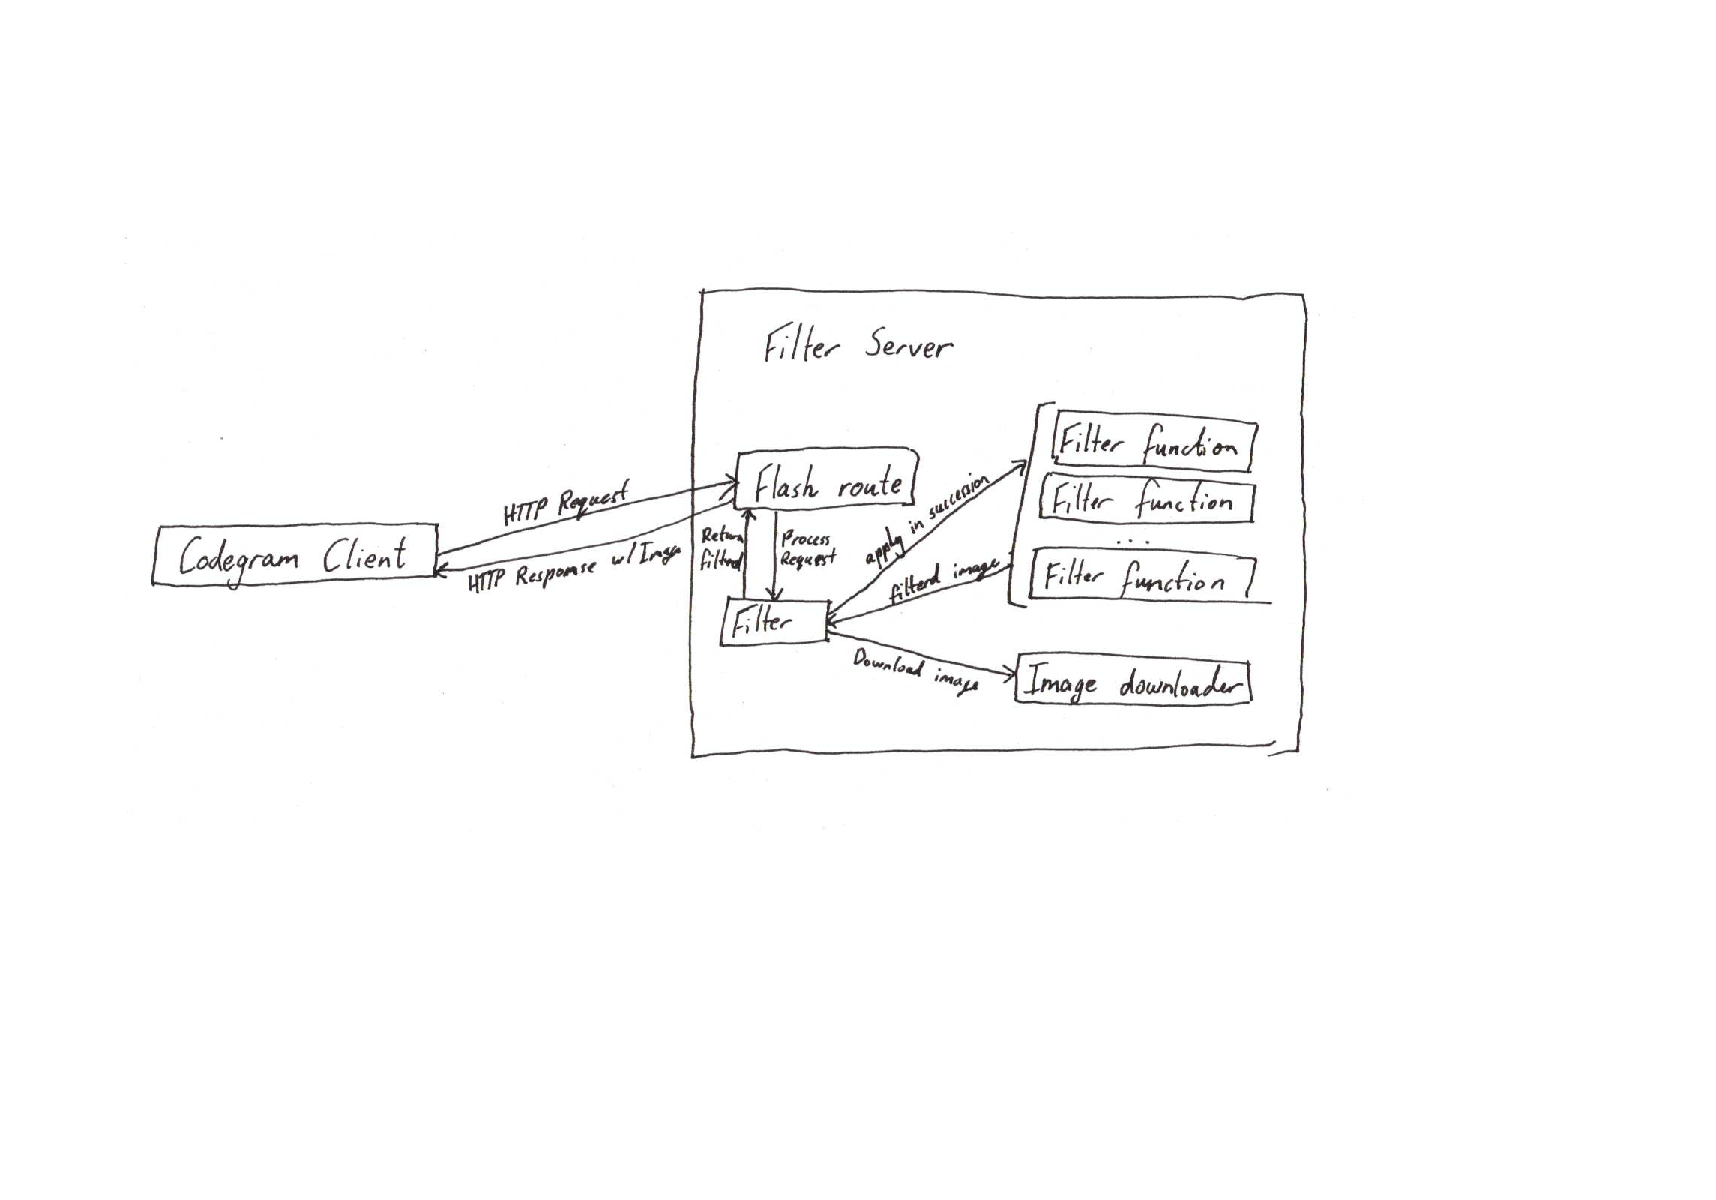
\includegraphics[width=0.8\textwidth]{diagram.pdf}
    \caption{Design Diagram}
    \label{fig:diagram}
\end{figure}

\section{Optimisation}

\paragraph{What are the time/computation consuming parts of your design?}
The time consuming parts of our design are the image processing steps.
This computation is inherent to the image filtering feature.
We have minimised the amount of web requests by batching the image processing steps into a single request.

\paragraph{Are there any bottlenecks?}
The bottleneck in our design is the image processing steps.
Again, this is inherent to the image filtering feature.

\paragraph{Are there any use cases that you can optimise?}
We currently optimise the use case where the user wants to apply multiple filters to the same image.

We could also optimise the use case where the user wants to apply the same filter to multiple images by including an array of images in the request.

We could optimise applying repeated filters by caching the results of the filters.

\paragraph{How would you scale your design to support more users?}
We would horizontally scale the image processing steps.
This would allow us to scale the image processing steps independently of the web server.
Adding filtering requests to a queue would also allow us to scale the web server independently of the image processing steps.

\paragraph{Are there any security concerns?}
Images are given to the filtering service as a public URL.
This means that all user images are publicly accessible,
which may be a security concern of the system but is not a concern of the image filtering feature.

\section{Design Challenges}

\subsection{Malicious Images}
As we process filtering steps in bulk,
the original image may be malicious.
We could, at the point of processing,
check the hash of the image to ensure that it is not malicious.
However, this does not account for applying the filter service multiple times.

Additionally, this is inflexible as our database of malicious images is likely to be updated frequently which is why Codegram does a periodic scan.
Instead we should store the hash pairs of the original and filtered images in a database.
This allows us to extend our malicious image detection to include hashes of filtered images.
However, this approach could be expensive as we could require a much larger malicious hash list.
We could instead store the hash of the original image with each filtered image and check this hash during the scan.

\subsection{Reordering Filters}
For most filters, the order in which they are applied does not matter.
This gives us the ability to improve the performance of repeated filter queries in different orders by caching the results of the filters.
One method of caching the results would be to sort the filters by name in the request and hash the resulting request,
then store a mapping from the hash to the filtered image.
This would allow us to quickly return the filtered image if the request is repeated in any order.

However, this approach does not work for filters that depend on the order in which they are applied.
As an obvious example, say we have an advanced filter that adds coloured party hats on each semi-colon in the image.
If we apply this filter before the grayscale filter, the hats will be coloured.
We would need to flag this filter as order dependent and not cache the results.
This could be done by a naming convention such as \texttt{order\_dependent\_party\_hats}.
Or we could keep a list of order dependent filters in the code.
This would limit the extensibility of the system so we need to consider the weigh the benefits based on what our system priorities are.


\subsection{Global Access}
To optimise for global access,
we can consider using a distributed system or a CDN to store and serve the filtered images.
This would allow users to access their images from a location close to them and reduce latency.

\section{Programming Challenge}

\begin{code}[language=python]{pipeline.py}
import cv2
import numpy as np
import requests
from flask import Flask, request, send_file

def read_image(url):
    response = requests.get(url)
    image = np.asarray(bytearray(response.content), dtype="uint8")
    image = cv2.imdecode(image, cv2.IMREAD_COLOR)
    return image

def brightness(image, amount):
    hsv = cv2.cvtColor(image, cv2.COLOR_BGR2HSV)
    hsv = np.array(hsv, dtype=np.float64)
    hsv[:, :, 1] = hsv[:, :, 1] * amount
    hsv[:, :, 1][hsv[:, :, 1] > 255] = 255
    hsv[:, :, 2] = hsv[:, :, 2] * amount
    hsv[:, :, 2][hsv[:, :, 2] > 255] = 255
    hsv = np.array(hsv, dtype=np.uint8)
    image = cv2.cvtColor(hsv, cv2.COLOR_HSV2BGR)
    return image

def contrast(image, amount):
    image = np.array(image, dtype=np.float64)
    image = (image - 128) * amount + 128
    image[image > 255] = 255
    image[image < 0] = 0
    image = np.array(image, dtype=np.uint8)
    return image

def saturation(image, amount):
    hsv = cv2.cvtColor(image, cv2.COLOR_BGR2HSV)
    hsv = np.array(hsv, dtype=np.float64)
    hsv[:, :, 1] = hsv[:, :, 1] * amount
    hsv[:, :, 1][hsv[:, :, 1] > 255] = 255
    hsv = np.array(hsv, dtype=np.uint8)
    image = cv2.cvtColor(hsv, cv2.COLOR_HSV2BGR)
    return image

def grayscale(image):
    return cv2.cvtColor(image, cv2.COLOR_BGR2GRAY)

def sepia(image):
    return cv2.transform(image, np.matrix([[0.272, 0.534, 0.131],
                                           [0.349, 0.686, 0.168],
                                           [0.393, 0.769, 0.189]]))

def blur(image, kernel_size):
    return cv2.blur(image, (kernel_size, kernel_size))

def pipeline(image, filters):
    for filter_func, params in filters:
        image = filter_func(image, **params)
    return image

app = Flask(__name__)

@app.route('/filter', methods=['POST'])
def filter():
    data = request.get_json()
    image = read_image(data['image'])
    filters = [
        (globals()[filter['name']], filter['parameters'])
        for filter in data['filters']
    ]
    image = pipeline(image, filters)
    return send_file(cv2.imencode('.jpg', image)[1].tobytes(),
                     mimetype='image/jpeg')

if __name__ == '__main__':
    app.run()
\end{code}



\end{document}

